\section{Materials}
\label{sec:materials}

\subsection{Task and class definitions}
The task is single-label classification of a frontal chest radiograph into six mutually exclusive classes, in the fixed order COVID-19, Normal, Pleural Effusion, Pneumonia, Pulmonary Nodule/Mass and Tuberculosis. Images carrying more than one of these findings are excluded where the source makes this visible (Section~\ref{sec:labels}); the single-label assumption is a limitation discussed in Section~\ref{sec:limitations}.

\subsection{Sources and acquisition}
\label{sec:sources}
Table~\ref{tab:sources} lists the sources. Each was downloaded from its official distribution point by an acquisition script that resumes interrupted transfers, compares the final size with the server's \texttt{Content-Length} header, rejects HTML error pages returned in place of data, and appends one provenance record per file (URL, start and end time, size in bytes and SHA-256 digest) to a per-source log. Where the publisher provides a checksum (MD5 entity tags for the NLM sets, a published digest for the Kermany archive) it was verified. The COVID-19 image data collection was obtained as a Git clone and is identified by its commit hash. Two sources that the original design included, VinDr-CXR~\cite{nguyen2022vindr} and JSRT~\cite{shiraishi2000development}, require credentialed access or registration and were not used. A TB archive aggregated from several hospitals~\cite{rahman2020reliable}, which was used in the earlier V5 pipeline, was excluded because it is described as containing NLM Montgomery images, our external cohort, without the original identifiers; it was replaced by the official Shenzhen set.

\begin{table}[t]
\centering
\caption{Data sources, their role, the classes they contribute and the patient-identity status used for grouping. Licence terms were not verified for this manuscript; ``see source terms'' means that the publisher's terms must be read before reuse. The images are not redistributed.}
\label{tab:sources}
\small
\begin{tabular}{@{}p{3.0cm}p{1.5cm}p{3.6cm}p{2.4cm}p{3.2cm}@{}}
\toprule
Source & Builds & Classes contributed & Patient identity & Licence / terms \\
\midrule
NIH ChestX-ray14~\cite{wang2017chestxray8} & 1, 2 & Normal, Pleural Effusion, Nodule/Mass, Pneumonia & Genuine (patient ID) & See source terms \\
Kermany et al., Mendeley v2~\cite{kermany2018identifying} & 1, 2 & Normal, Pneumonia (paediatric) & Derived from file name & See source terms \\
Shenzhen (NLM)~\cite{jaeger2014two,candemir2014lung} & 1, 2 & Normal, Tuberculosis & One image per subject & See source terms (NLM) \\
COVID-19 image data collection~\cite{cohen2020covid} & 1, 2 & COVID-19, Pneumonia, Normal, Tuberculosis & Genuine (collection patient ID) & See source terms (per image) \\
TBX11K~\cite{liu2020rethinking} & 2 & Normal, Tuberculosis & Unknown (grouped per image) & See source terms \\
COVID-19 Radiography Database~\cite{chowdhury2020can,rahman2021exploring} & 2 & COVID-19 & Unknown (grouped per image) & See source terms \\
Montgomery County (NLM)~\cite{jaeger2014two,candemir2014lung} & external & Normal vs Tuberculosis (binary) & One image per subject & See source terms (NLM) \\
\bottomrule
\end{tabular}
\end{table}

\subsection{Labelling rules}
\label{sec:labels}
All labelling rules were written into a versioned configuration file before any V6 training and were not changed afterwards (configuration SHA-256 \texttt{b839fdbb\ldots}, recorded in both build reports). Labels come only from each source's own labels; an image is never labelled by the name of the archive it came from. Every included image records the identifier of the rule that labelled it, and every excluded image records the reason.

\begin{itemize}
\item \textbf{NIH ChestX-ray14.} Exactly one finding: \emph{Effusion} $\rightarrow$ Pleural Effusion; \emph{Nodule} and/or \emph{Mass} and nothing else $\rightarrow$ Pulmonary Nodule/Mass; \emph{Pneumonia} $\rightarrow$ Pneumonia; \emph{No Finding} $\rightarrow$ Normal, with at most one image per patient. Images with any other or additional finding are excluded. These labels are mined from reports by natural-language processing, not read from the images~\cite{wang2017chestxray8,oakdenrayner2020exploring}.
\item \textbf{Kermany.} \emph{NORMAL} $\rightarrow$ Normal; \emph{PNEUMONIA} (bacterial or viral) $\rightarrow$ Pneumonia. The population is paediatric.
\item \textbf{Shenzhen.} File-name suffix \texttt{\_0} $\rightarrow$ Normal; \texttt{\_1} (TB manifestation on clinical reading) $\rightarrow$ Tuberculosis.
\item \textbf{TBX11K.} \emph{Healthy} $\rightarrow$ Normal; \emph{active TB only} $\rightarrow$ Tuberculosis. ``Sick but non-TB'' images are excluded, because the cause of the abnormality is not specified and is not evidence of pneumonia; images with any latent-TB annotation are excluded, because latent TB is not an active-TB radiographic label; official test images without public labels are not used.
\item \textbf{COVID-19 image data collection.} Frontal radiographs (PA or AP) only, with finding containing \emph{COVID-19} $\rightarrow$ COVID-19; finding starting with \emph{Pneumonia} and not containing COVID-19 $\rightarrow$ Pneumonia; \emph{Tuberculosis} $\rightarrow$ Tuberculosis; \emph{No Finding} $\rightarrow$ Normal. Lateral views, computed tomography and other findings are excluded.
\item \textbf{COVID-19 Radiography Database.} Images in the COVID folder $\rightarrow$ COVID-19; the other folders are not used.
\item \textbf{Montgomery County.} \texttt{\_0} $\rightarrow$ normal, \texttt{\_1} $\rightarrow$ TB; used only as an external binary cohort.
\end{itemize}

\subsection{Content hashing and near-duplicate detection}
\label{sec:hashing}
For every image the builder computes the MD5 and SHA-256 digests of the raw file and a 64-bit perceptual hash (pHash) from the discrete cosine transform of a downscaled grey-level image. Let $h_i\in\{0,1\}^{64}$ be the pHash of image $i$ and $\mathbf{t}_i\in\mathbb{R}^{4096}$ its $64\times64$ grey-level thumbnail, flattened and normalised to unit length. Two images $i,j$ are declared near-duplicates when
\begin{equation}
d_H(h_i,h_j)=\sum_{b=1}^{64}\left[h_{i,b}\neq h_{j,b}\right]\le 6
\quad\text{and}\quad
\rho_{ij}=\mathbf{t}_i^{\top}\mathbf{t}_j\ge 0.97 .
\label{eq:neardup}
\end{equation}
The Hamming test is a cheap candidate filter; the thumbnail correlation confirms the match and rejects pairs that share a coarse layout only, which is common among chest radiographs. The comparison runs across all sources, including the external cohort.

\subsection{Per-source caps}
To bound CPU training time and to stop a single source from dominating a class, the number of images per (source, class) pair was capped before splitting. Capping samples whole patient groups with a fixed seed (20261102). The caps were: NIH Normal 1,200, NIH Pleural Effusion 3,000 and NIH Nodule/Mass 3,000 (NIH Pneumonia uncapped); Kermany Normal 1,000 and Pneumonia 2,200; TBX11K Normal 1,000 (Tuberculosis uncapped); COVID-19 Radiography Database COVID-19 2,500; Shenzhen and the COVID-19 image data collection uncapped.

\subsection{Patient grouping, split and leakage checks}
\label{sec:split}
The unit of partitioning is the \emph{patient group}. The base group is the genuine patient identifier where the source provides one (NIH, COVID-19 image data collection), an identifier derived from the file name where possible (Kermany, whose file names carry a person token), one subject per image where the publisher documents one image per subject (Shenzhen, Montgomery), and otherwise a group of one image (TBX11K, COVID-19 Radiography Database). Groups are then merged by union--find over every pair of images that share an MD5 digest or satisfy Eq.~\eqref{eq:neardup}. Exact and near-duplicates can therefore never fall into different splits.

Whole groups are assigned to training, validation and internal test at a target ratio of 70/15/15, stratified by each group's majority (class, source) pair, using a fixed seed and greedy filling toward the target image counts. The Montgomery set has the role \emph{external} and is never part of a development split; any development image that matches a Montgomery image by MD5 or by Eq.~\eqref{eq:neardup} is excluded, not merely kept out of the test split. The \emph{split fingerprint} is the SHA-256 of the sorted list of \texttt{image\_id<TAB>split} lines; it is written into the build report, every training record and every evaluation report, so that a result can be traced to the exact partition.

The build report records three leakage checks: the number of patient groups present in more than one split, the number of identical files (MD5) present in more than one split, and the number of external-cohort files present in the development data. All three are zero for both builds (Table~\ref{tab:builds}). The first check proves patient-level separation only for rows with known patient identity; for TBX11K and the COVID-19 Radiography Database, patient identity is unknown, those images are grouped per image (plus merged duplicates), and the same patient could still appear in two splits.

\subsection{The two dataset builds}
\label{sec:builds}
Two builds were produced with the same rules. Build~1 (\texttt{v6\_build\_001}) used the five sources that had been downloaded at the time: NIH ChestX-ray14, Kermany, Shenzhen, the COVID-19 image data collection and Montgomery (external). In build~1 every COVID-19 image therefore comes from a single collection of images taken from publications and websites, and almost all Tuberculosis images come from Shenzhen. Build~2 (\texttt{v6\_build\_002}) adds TBX11K and the COVID-19 Radiography Database, giving COVID-19 and Tuberculosis a second source each, and two NIH image archives that were not yet available locally for build~1. Tables~\ref{tab:builds}--\ref{tab:sourcesplit} give the composition of both builds; Fig.~\ref{fig:composition} shows the final build graphically. The model reported in Section~\ref{sec:results} was trained on build \RDatasetBuild, with $N_{\text{train}}=\RNTrain$, $N_{\text{val}}=\RNVal$, $N_{\text{test}}=\RNTest$ and $N_{\text{external}}=\RNExternal$.

% Dataset counts below are copied from the build reports (not model results):
%   data/derived/v6_build_001/v6_build_report.json  (split_fingerprint 872abd3b...56cb, generated 2026-11-02T22:26:21Z)
%   data/derived/v6_build_002/v6_build_report.json  (split_fingerprint 5973233f...a7dfa5, generated 2026-11-03T04:37:23Z)
\begin{table}[t]
\centering
\caption{Images per class and split in the two V6 builds, with build-level checks. Counts are copied from the build reports (\texttt{v6\_build\_report.json}); split fingerprints are abbreviated.}
\label{tab:builds}
\small
\begin{tabular}{@{}lrrrrrr@{}}
\toprule
 & \multicolumn{3}{c}{Build 1 (\texttt{v6\_build\_001})} & \multicolumn{3}{c}{Build 2 (\texttt{v6\_build\_002})} \\
\cmidrule(lr){2-4}\cmidrule(lr){5-7}
Class & Train & Val & Test & Train & Val & Test \\
\midrule
COVID-19                & 334   & 73    & 71    & 2,083  & 444   & 451 \\
Normal                  & 1,477 & 308   & 314   & 2,152  & 464   & 467 \\
Pleural Effusion        & 2,112 & 448   & 440   & 2,099  & 457   & 444 \\
Pneumonia               & 1,804 & 390   & 391   & 1,829  & 394   & 394 \\
Pulmonary Nodule/Mass   & 2,085 & 458   & 457   & 2,110  & 441   & 449 \\
Tuberculosis            & 242   & 54    & 51    & 684    & 148   & 145 \\
\midrule
Total                   & 8,054 & 1,731 & 1,724 & 10,957 & 2,348 & 2,350 \\
\midrule
External (Montgomery)   & \multicolumn{3}{c}{80 normal, 58 TB} & \multicolumn{3}{c}{80 normal, 58 TB} \\
Patient identity: genuine / filename / unknown & \multicolumn{3}{c}{8,844 / 2,665 / 0} & \multicolumn{3}{c}{8,882 / 2,643 / 4,130} \\
Near-duplicate pairs merged & \multicolumn{3}{c}{39} & \multicolumn{3}{c}{545} \\
Groups / files spanning splits & \multicolumn{3}{c}{0 / 0} & \multicolumn{3}{c}{0 / 0} \\
External files in development & \multicolumn{3}{c}{0} & \multicolumn{3}{c}{0} \\
Split fingerprint & \multicolumn{3}{c}{\texttt{872abd3b\ldots}} & \multicolumn{3}{c}{\texttt{5973233f\ldots}} \\
\bottomrule
\end{tabular}
\end{table}

\begin{table}[t]
\centering
\caption{Images per source and split in the two V6 builds, and the number of source images excluded by the labelling rules, caps or decoding checks. Counts from the build reports.}
\label{tab:sourcesplit}
\small
\begin{tabular}{@{}lrrrrrrrr@{}}
\toprule
 & \multicolumn{4}{c}{Build 1} & \multicolumn{4}{c}{Build 2} \\
\cmidrule(lr){2-5}\cmidrule(lr){6-9}
Source & Train & Val & Test & Excl. & Train & Val & Test & Excl. \\
\midrule
NIH ChestX-ray14              & 5,240 & 1,123 & 1,121 & 87,515 & 5,270 & 1,128 & 1,124 & 104,598 \\
Kermany                       & 1,863 & 402   & 400   & 4,710  & 1,848 & 397   & 398   & 4,732 \\
Shenzhen                      & 463   & 100   & 99    & 0      & 463   & 100   & 99    & 0 \\
COVID-19 image data coll.     & 488   & 106   & 104   & 252    & 493   & 94    & 111   & 252 \\
TBX11K                        & --    & --    & --    & --     & 1,141 & 245   & 244   & 6,770 \\
COVID-19 Radiography DB       & --    & --    & --    & --     & 1,742 & 384   & 374   & 1,116 \\
\bottomrule
\end{tabular}
\end{table}

The largest exclusion categories in build~2 were NIH images with another or an additional finding (42,242), NIH \emph{No Finding} images beyond one per patient (35,454), images not sampled because of a cap (34,993 in total over all capped pairs), TBX11K ``sick but non-TB'' images (3,800), undecodable or very small images (557), TBX11K latent or unknown TB annotations (169) and COVID-19 image data collection images that were not frontal radiographs (168) or carried a finding outside the six classes (84). The corresponding build~1 figures are in its build report.

\begin{figure}[t]
\centering
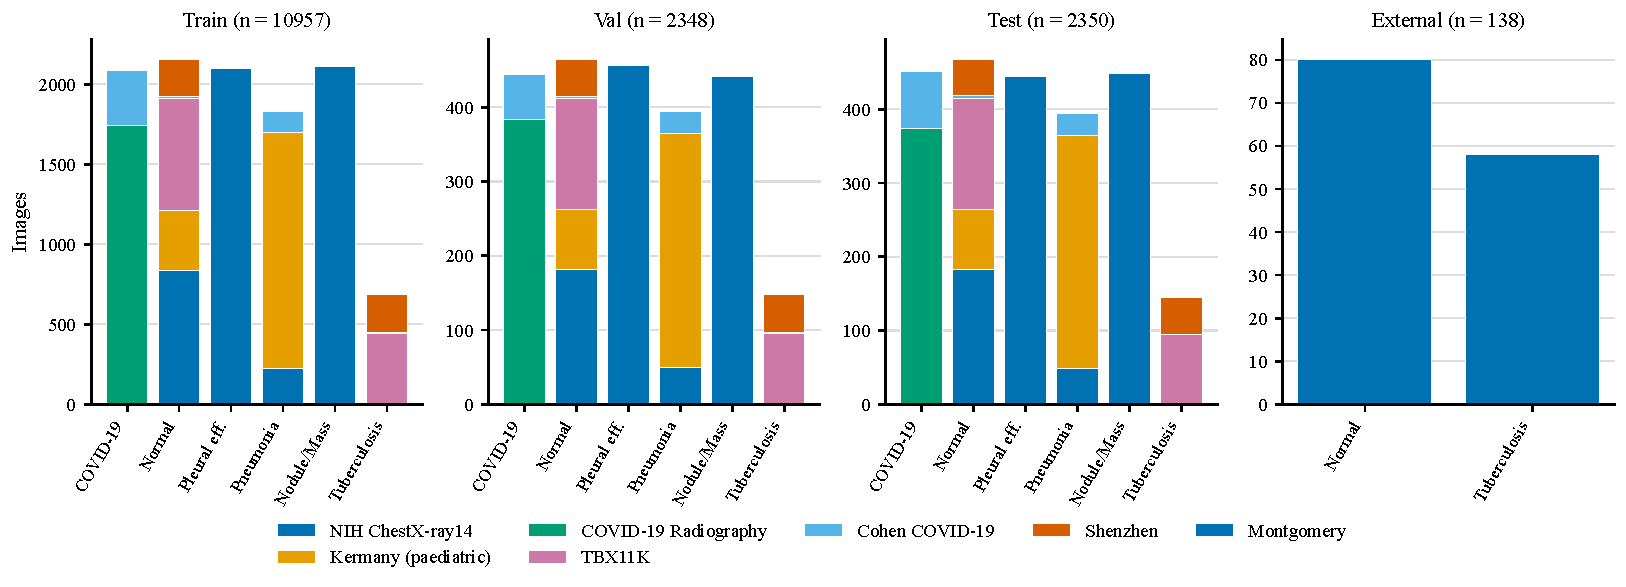
\includegraphics[width=\linewidth]{fig_dataset_composition.pdf}
\caption{Images per class and source in the training, validation and test splits of the dataset build used for the reported model (\RDatasetBuild). Generated from the build manifest.}
\label{fig:composition}
\end{figure}

\subsection{External cohort}
The Montgomery County set contains 138 frontal radiographs from a United States county TB control programme: 80 normal and 58 with TB manifestations~\cite{jaeger2014two,candemir2014lung}. It shares no source with the development data, was never used for training or checkpoint selection and was evaluated once per run; Section~\ref{sec:design} gives the caveat that run~2 was started after run~1's external results had been seen. It contains only normal and TB images, so it tests whether the classifier separates abnormal from normal radiographs from an unseen hospital, and whether it names TB correctly; it does not test six-class accuracy.
